\section{Correction using timing beacon on satellite}
The timing beacon correction method installs a beacon with regular pulses on the satellite. We time-stamp the beacon signal both on the satellite and at the ground station (Fig \ref{fig:beacon}). If we find the cross correlation between the beacon pulses registered on the satellite timestamp and those registered on the ground station, we can apply the same transformation to the idler and signal photoevents. We find that even a high jitter beacon with poor detection efficiency is sufficient to correct for all clock drifts including the change of the Doppler shift for high elevation angles.

\begin{figure}[ht!]
	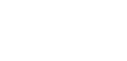
\includegraphics[width=0.97\linewidth]{assets/beacon}
	\caption{The time-stamping units and beacon generator use the same clock reference.}
	\label{fig:beacon}
\end{figure}

\subsection{Cross-correlation using FFT}
